
\documentclass{exam}

\usepackage{units} 
\usepackage{graphicx}
\usepackage[fleqn]{amsmath}
\usepackage{cancel}
\usepackage{float}
\usepackage{mdwlist}
\usepackage{booktabs}
\usepackage{cancel}
\usepackage{polynom}
\usepackage{caption}
\usepackage{fullpage}
\usepackage{xfrac}
\usepackage{enumerate}

\newcommand{\degree}{\ensuremath{^\circ}} 
\everymath{\displaystyle}

% \begin{figure}[H]
%   \centering
%   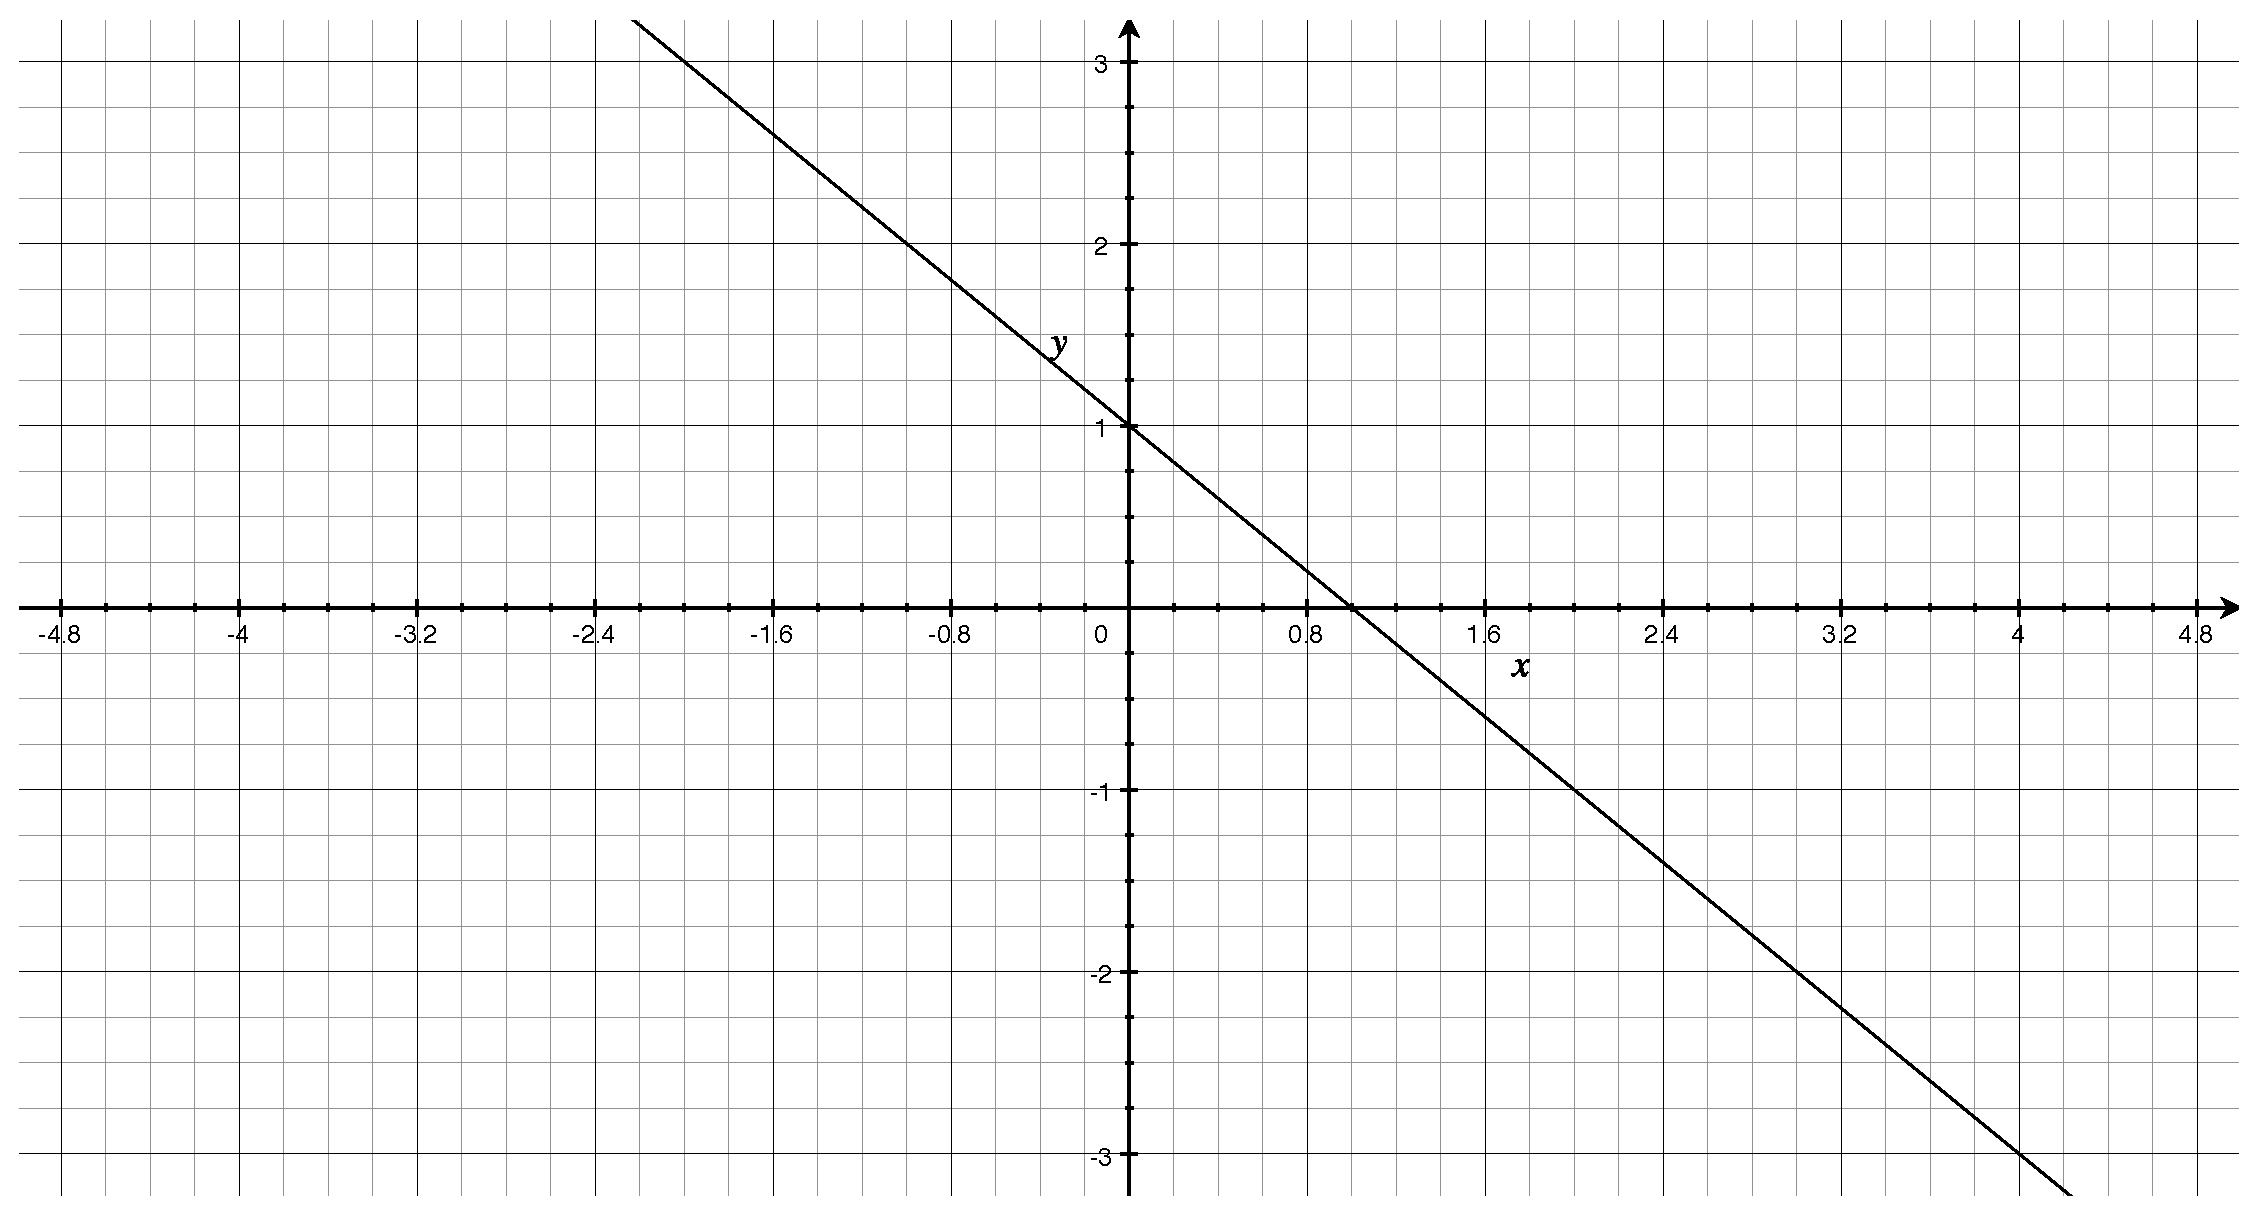
\includegraphics[scale=.3]{problem7.eps}
%   \caption*{Problem 7}
% \end{figure}

% \begin{tabular}{cc}
%   \toprule
%   period & amplitude \\
%   \midrule
%   value one & value two
%   \bottomrule
% \end{tabular}

\printanswers

\ifprintanswers 
  \usepackage{2in1, lscape} 
\fi

\date{May 15, 2013}
\author{}
\title{Math 141 \\ Homework 12}

\begin{document}

\maketitle

\section{Administrative}

The Chapter 3 test will be next week (May 22).  You should prepare for the test by doing the chapter review problems and
sample test at the end of the chapter.  

\section{Homework}

\begin{itemize*}
  \item Read Section 3.6 
  \item Section 3.6: 5-32, 36-39, 46-49, 55-64, 81
\end{itemize*}

\section{Extra Credit}
Section 3.6: 82 and 84

\ifprintanswers
  \pagebreak

  \begin{description}
    \item[82]
      \begin{itemize*}
        \item there is no x-intercept because the numerator has no real solution
        \item there is no horizontal asymptote because the numerator is higher degree than the denominator
        \item there is no vertical asymptote because the denominator has no real solution
        \item there is no slant asymptote because the degree of the numerator is not exactly one greater than the degree
          of the denominator
        \item since all the powers are even and the degree of the numerator is greater than the degree of the
          denominator, the function's value is always positive and the values get bigger and bigger as 
          $x \rightarrow \pm \infty$.
      \end{itemize*}

      \begin{figure}[H]
        \centering
        \includegraphics{problem82.eps}
        \caption*{Problem 82: $r(x) = \frac{x^6 + 10}{x^4 + 8x^2 + 15}$}
      \end{figure}

    \pagebreak

    \item[84]
      \begin{enumerate}[a]

        \item 
          This is the graph of $f(x) = \frac{1}{x^2}$ shifted right by 2.

          \begin{figure}[H]
            \centering
            \includegraphics{problem84a.eps}
            \caption*{Problem 84a: $r(x) = \frac{1}{(x - 2)^2}$}
          \end{figure}

        \item
          % \[ \polylongdiv{2x^2 + 4x + 5}{x^2 + 2x + 1} \]

          \[
            \frac{2x^2 + 4x + 5}{x^2 + 2x + 1} = 2 + \frac{3}{(x + 1)^2}
          \]
          This graph is the graph of $\frac{1}{x^2}$ scaled vertically 3, shifted left by 1, up 2, and 

          \begin{figure}[H]
            \centering
            \includegraphics{problem84b.eps}
            \caption*{Problem 84b: $r(x) = \frac{2x^2 + 4x + 5}{x^2 + 2x + 1}$}
          \end{figure}

        \item
          After doing long division, you find that:
          \begin{align*}
            \frac{2 - 3x^2}{x^2 - 4x + 4} &= -3 + \frac{-12x + 14}{(x - 2)^2} \\
            \frac{12x - 3x^2}{x^2 - 4x + 4} &= -3 + \frac{1}{(x - 2)^2} \\
          \end{align*}

          Only the second function can be written as a transformation of $f(x) = \frac{1}{x^2}$.  
      \end{enumerate}

  \end{description}

  \pagebreak

  \section{Section 3.6}

  \begin{description}

    \item[5] 
      $f(x) = \frac{x - 1}{x + 4}$ 

      \begin{itemize*}
        \item x-intercept: $(1, 0)$
        \item y-intercept: $\left(0, -\frac{1}{4} \right)$
      \end{itemize*}

    \item[6] 
      $f(x) = \frac{3x}{x - 5}$ 

      \begin{itemize*}
        \item x-intercept: $(0, 0)$
        \item y-intercept: $(0, 0)$
      \end{itemize*}

    \item[7] 
      $f(x) = \frac{x^2 - x - 2}{x - 6}$ 

      \begin{align*}
        x^2 - x - 2    &= 0 \\
        (x - 2)(x + 1) &= 0 \\
        x &= \left\{ -1, 2 \right\} \\
      \end{align*}

      \begin{itemize*}
        \item x-intercept: $(-1, 0), (2, 0)$
        \item y-intercept: $\left( 0, \frac{1}{3} \right)$
      \end{itemize*}

    \item[8] 
      $f(x) = \frac{2}{x^2 + 3x - 4}$ 

      \begin{itemize*}
        \item x-intercept: none
        \item y-intercept: $\left( 0, -\frac{1}{2} \right)$
      \end{itemize*}

    \pagebreak

    \item[9] $f(x) = \frac{x^2 - 9}{x^2}$ 
      \begin{align*}
        x^2 - 9 &= 0 \\
        (x - 3)(x + 3) &= 0 \\
        x &= \left\{ -3, 3 \right\} \\
      \end{align*}

      \begin{itemize*}
        \item x-intercept: $(-3, 0)$, $(3, 0)$
        \item y-intercept: none
      \end{itemize*}

    \item[10] $f(x) = \frac{x^3 + 8}{x^2 + 4}$ 
      \begin{itemize}
        \item x-intercept: $(-2, 0)$
        \item y-intercept: $(0, 2)$
      \end{itemize}

    \item[11] 
      \begin{itemize}
        \item x-intercept: $(3, 0)$
        \item y-intercept: $(0, 3)$
        \item vertical asymptote: $x = 2$
        \item horizontal asymptote: $y = 2$
      \end{itemize}

    \item[12] 
      \begin{itemize}
        \item x-intercept: $(0, 0)$
        \item y-intercept: $(0, 0)$
        \item vertical asymptote: $x = -1$, $x = 2$
        \item horizontal asymptote: $y = 0$
      \end{itemize}

    \item[13] 
      \begin{itemize}
        \item x-intercept: $(-1, 0)$ and $(1, 0)$
        \item y-intercept: $\left( 0, \frac{1}{4} \right)$
        \item vertical asymptote: $x = -2$ and $x = 2$
        \item horizontal asymptote: $y = 1$
      \end{itemize}

    \item[14] 
      \begin{itemize}
        \item x-intercepts: $(-2, 0), (2, 0)$
        \item y-intercept: $\left( 0, -6 \right)$
        \item no vertical asymptote
        \item horizontal asymptote: $y = 2$
      \end{itemize}

    \pagebreak

    \item[15] 
      \begin{itemize*}
        \item vertical asymptote: $x = -2$
        \item horizontal asymptote: $y = 0$
      \end{itemize*}

    \item[16] 
      \begin{itemize*}
        \item vertical asymptote: $x = 1$
        \item horizontal asymptote: $y = 2$
      \end{itemize*}

    \item[17] 
      \begin{align*}
        x^2 - x - 6    &= 0 \\
        (x - 3)(x + 2) &= 0 \\
        x              &= \left\{ -2, 3 \right\} \\
      \end{align*}

      \begin{itemize*}
        \item vertical asymptote: $x = -2$ and $x = 3$
        \item horizontal asymptote: $y = 1$
      \end{itemize*}

    \item[18] 
      \begin{align*}
       x^2 + 2x + 1 &= 0 \\
        (x + 1)^2   &= 0 \\
        x           &= -1 \\
      \end{align*}

      \begin{itemize*}
        \item vertical asymptote: $x = -1$
        \item horizontal asymptote: $y = 0$
      \end{itemize*}

    \item[19] 
      \begin{itemize*}
        \item vertical asymptote: none
        \item horizontal asymptote: $y = 0$
      \end{itemize*}

    \item[20] 
      \begin{align*}
       (x - 3)(x - 4) &= 0 \\
       x              &= \left\{ 3, 4 \right\} \\
      \end{align*}

      \begin{itemize*}
        \item vertical asymptote: $x = 3$ and $x = 4$
        \item horizontal asymptote: $y = 1$
      \end{itemize*}

    \item[21] 
      \begin{align*}
       x^2 + 5x - 6    &= 0 \\
        (x + 6)(x - 1) &= 0 \\
        x              &= \left\{ -6, 1 \right\} \\
      \end{align*}

      \begin{itemize*}
        \item vertical asymptote: $x = -6$ and $x = 1$
        \item horizontal asymptote: $y = 0$
      \end{itemize*}

    \item[22] 
      \begin{itemize*}
        \item vertical asymptote: none
        \item horizontal asymptote: $y = 3$
      \end{itemize*}

    \item[23] 
      \begin{itemize*}
        \item vertical asymptote: $x = 1$
        \item horizontal asymptote: none
      \end{itemize*}

    \item[24] 
      \begin{align*}
       (x^2 - 4)       &= 0 \\
        (x + 2)(x - 2) &= 0 \\
        x              &= \left\{ -2, 2 \right\} \\
      \end{align*}

      \begin{itemize*}
        \item vertical asymptote: $x = -2$ and $x = 2$
        \item horizontal asymptote: none
      \end{itemize*}

    \item[25] 
      \begin{figure}[H]
        \centering
        \includegraphics{problem25.eps}
        \caption*{Problem 25: $r(x) = \frac{1}{x - 1}$}
      \end{figure}

    \item[26] 
      \begin{figure}[H]
        \centering
        \includegraphics{problem26.eps}
        \caption*{Problem 26: $r(x) = \frac{1}{x + 4}$}
      \end{figure}

    \item[27] 
      \begin{figure}[H]
        \centering
        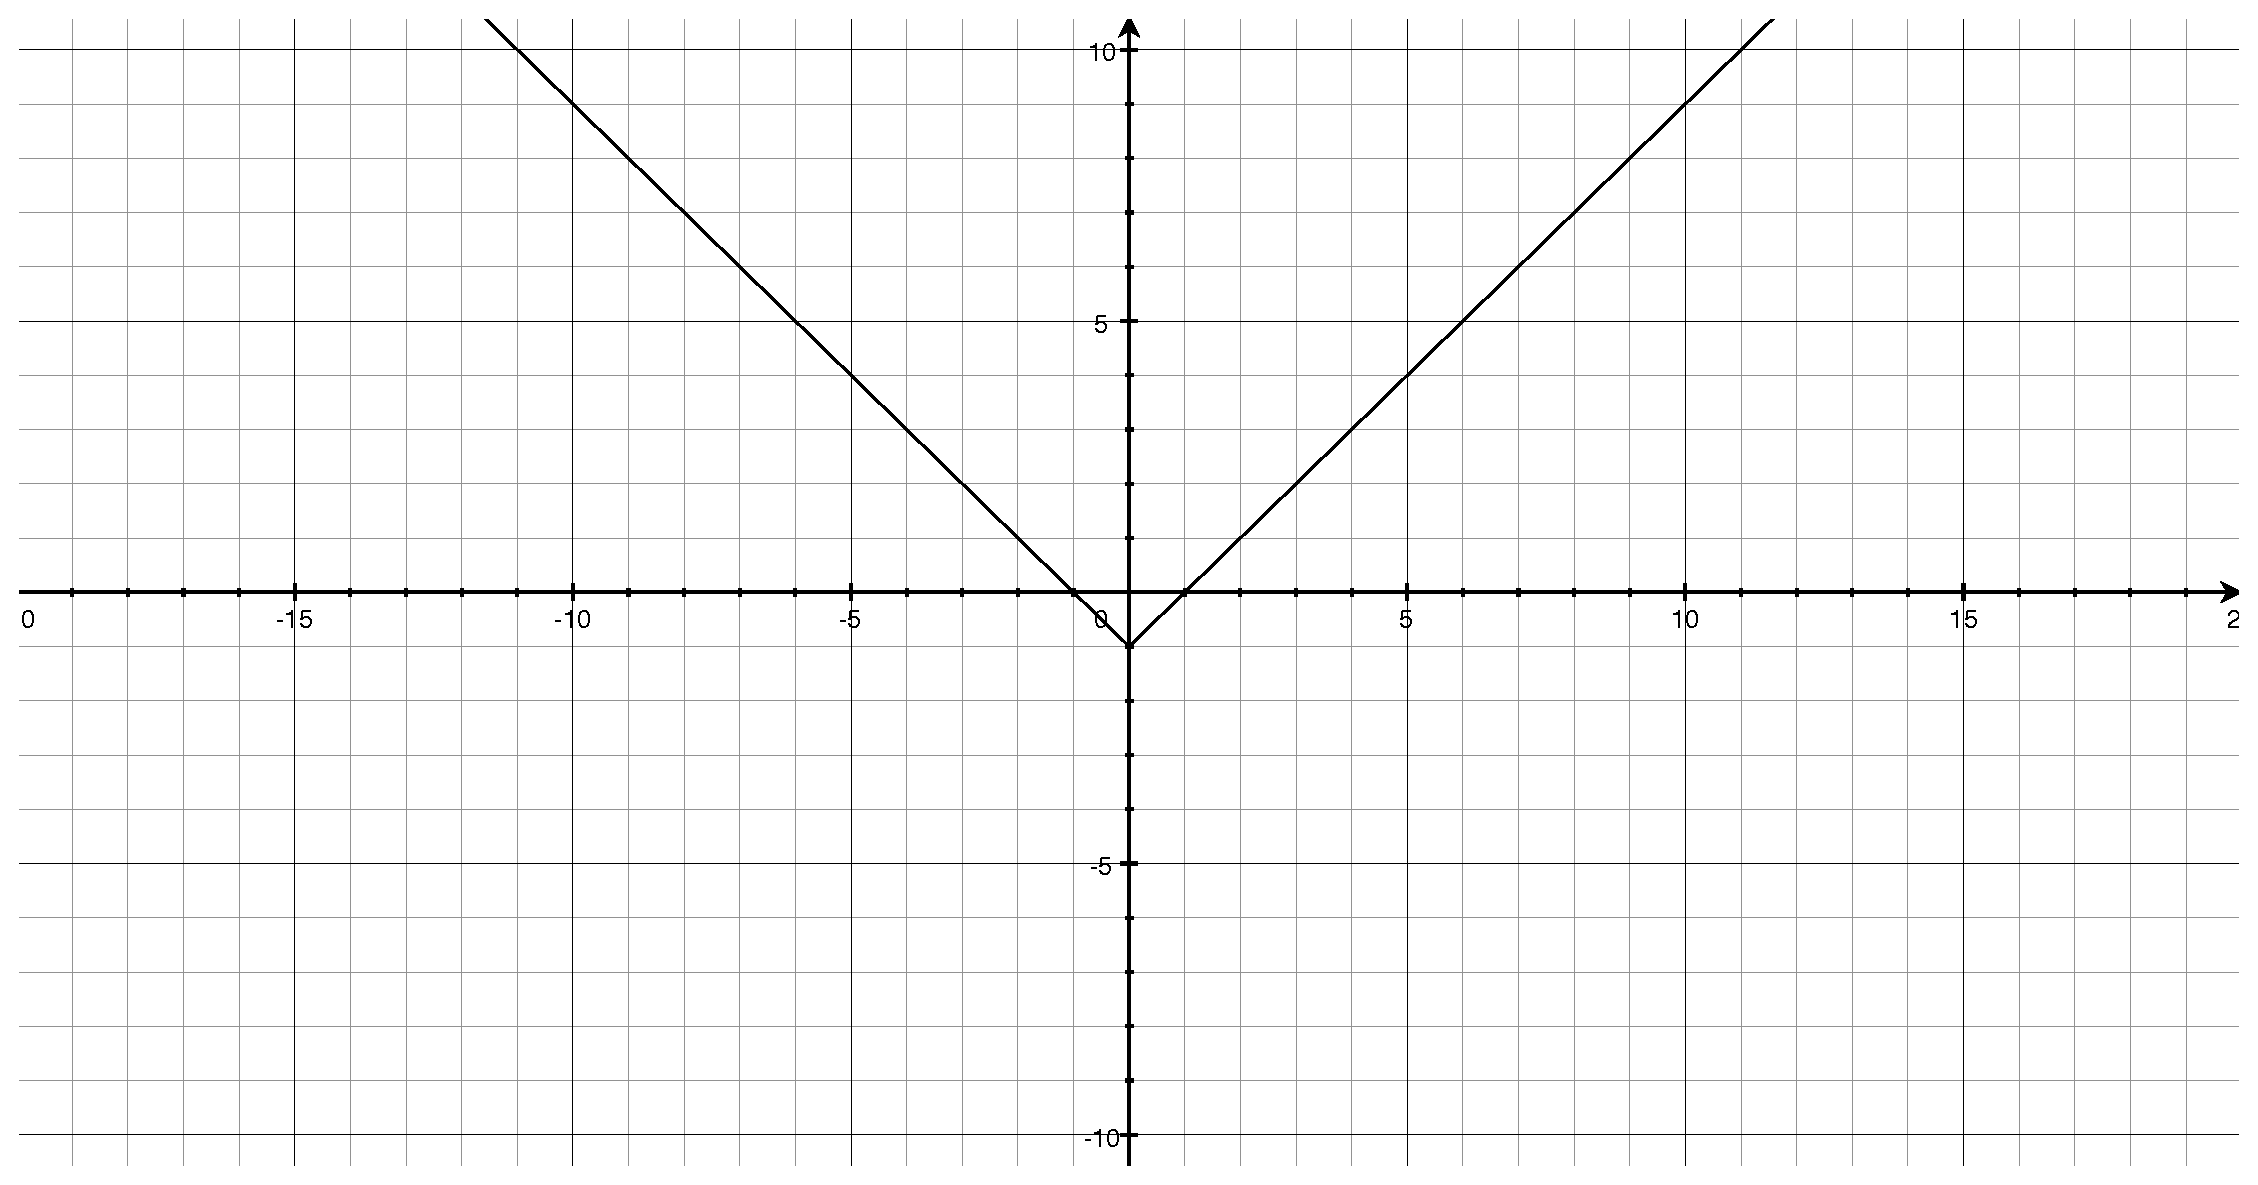
\includegraphics{problem27.eps}
        \caption*{Problem 27: $s(x) = \frac{3}{x + 1}$}
      \end{figure}

    \item[28] 
      \begin{figure}[H]
        \centering
        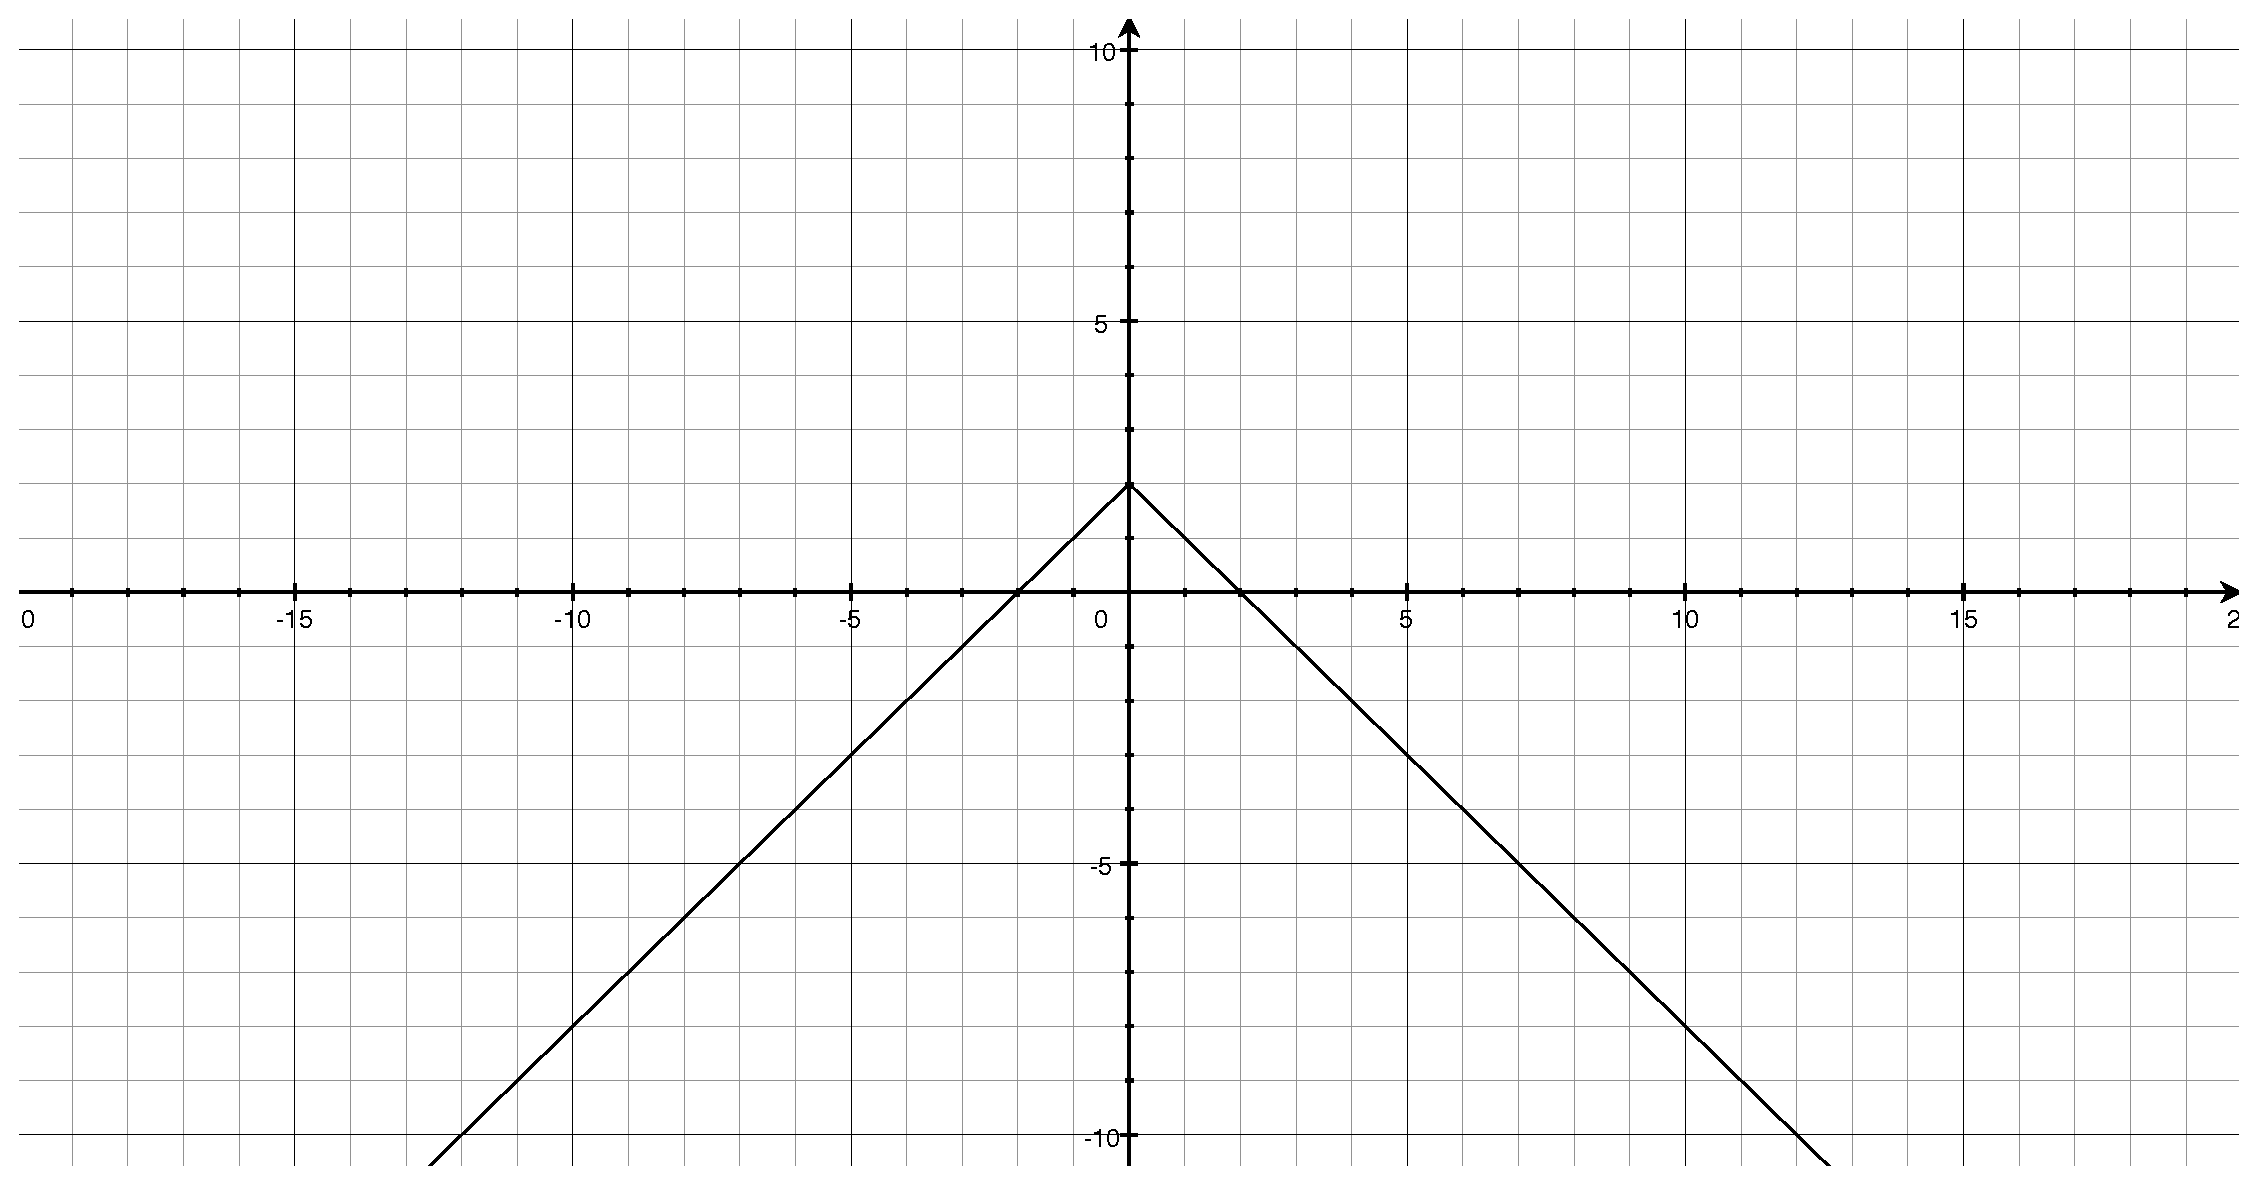
\includegraphics{problem28.eps}
        \caption*{Problem 28: $s(x) = \frac{-2}{x - 2}$}
      \end{figure}

    \item[29] 
      \[ \frac{2x + 3}{x + 2} = 2 + \frac{1}{x - 2} \]

      \begin{figure}[H]
        \centering
        \includegraphics[scale = 0.9]{problem29.eps}
        \caption*{Problem 29: $s(x) = \frac{2x-3}{x-2}$}
      \end{figure}

    \item[30] 
      \[ \frac{3x + 3}{x + 2} = 3 - \frac{9}{x + 2} \]

      \begin{figure}[H]
        \centering
        \includegraphics[scale = 0.9]{problem30.eps}
        \caption*{Problem 30: $t(x) = \frac{3x + 3}{x + 2}$}
      \end{figure}

    \item[31] 
      \[ \frac{x + 2}{x + 3} = 1 - \frac{1}{x + 3} \]

      \begin{figure}[H]
        \centering
        \includegraphics[scale = 0.9]{problem31.eps}
        \caption*{Problem 31: $t(x) = \frac{x + 2}{x + 3}$}
      \end{figure}

    \item[32] 
      \[ \frac{2x - 9}{x - 4} = 2 - \frac{1}{x - 4} \]

      \begin{figure}[H]
        \centering
        \includegraphics[scale = 0.9]{problem32.eps}
        \caption*{Problem 31: $t(x) = \frac{2x - 9}{x - 4}$}
      \end{figure}

    \item[36]
      \begin{tabular}{llll}
        \toprule
        x-intercept                     & y-intercept                     & vertical            & horizontal \\
                                        &                                 & asymptote           & asymptote \\
        \midrule
        $\left( \frac{1}{2}, 0 \right)$ & $\left( 0, \frac{1}{3} \right)$ & $x = - \frac{3}{2}$ & $y = -1$ \\
        \bottomrule
      \end{tabular}

      \begin{figure}[H]
        \centering
        \includegraphics[scale = 0.8]{problem36.eps}
        \caption*{Problem 36: $s(x) = \frac{1 - 2x}{2x + 3}$}
      \end{figure}

    \item[37]
      \begin{tabular}{llll}
        \toprule
        x-intercept & y-intercept & vertical  & horizontal \\
                    &             & asymptote & asymptote \\
        \midrule
        none        & $(0, 2)$    & $x = 3$   & $y = 0$ \\
        \bottomrule
      \end{tabular}

      \begin{figure}[H]
        \centering
        \includegraphics[scale = 0.8]{problem37.eps}
        \caption*{ Problem 37: $r(x) = \frac{18}{(x - 3)^2}$ }
      \end{figure}

    \item[38]
      \begin{tabular}{llll}
        \toprule
        x-intercept  & y-intercept & vertical  & horizontal \\
                     &             & asymptote & asymptote \\
        \midrule
        $(2, 0)$     & $(0, -2)$   & $x = -1$  & $y = 0$ \\
        \bottomrule
      \end{tabular}

      \begin{figure}[H]
        \centering
        \includegraphics[scale = 0.8]{problem38.eps}
        \caption*{ Problem 38: $r(x) = \frac{x - 2}{(x + 1)^2}$ }
      \end{figure}

    \item[39]
      \begin{tabular}{llll}
        \toprule
        x-intercept   & y-intercept & vertical          & horizontal \\
                      &             & asymptote         & asymptote \\
        \midrule
        $(2, 0)$      & $(0, 2)$    & $x = -1$, $x = 4$ & $y = 0$ \\
        \bottomrule
      \end{tabular}

      \begin{figure}[H]
        \centering
        \includegraphics[scale = 0.8]{problem39.eps}
        \caption*{ Problem 39: $r(x) = \frac{x - 2}{(x + 1)^2}$ }
      \end{figure}

    % \item[45]
    %   \begin{tabular}{llll}
    %     \toprule
    %     x-intercept         & y-intercept                     & vertical          & horizontal \\
    %                         &                                 & asymptote         & asymptote \\
    %     \midrule
    %     $(-2, 0)$, $(1, 0)$ & $\left( 0, \frac{2}{3} \right)$ & $x = -1$, $x = 3$ & $y = 1$ \\
    %     \bottomrule
    %   \end{tabular}

      % \begin{figure}[H]
      %   \centering
      %   \includegraphics[scale = 0.8]{problem45.eps}
      %   \caption*{ Problem 45: $r(x) = \frac{(x - 1)(x + 2)}{(x + 1)(x - 3)}$ }
      % \end{figure}

    \item[46]
      \begin{tabular}{llll}
        \toprule
        x-intercept         & y-intercept & vertical          & horizontal \\
                            &             & asymptote         & asymptote \\
        \midrule
        $(-2, 0)$, $(0, 0)$  & $(0, 0)$    & $x = 1$, $x = 4$ & $y = 2$ \\
        \bottomrule
      \end{tabular}

      \begin{figure}[H]
        \centering
        \includegraphics[scale = 0.8]{problem46.eps}
        \caption*{ Problem 46: $r(x) = \frac{2x(x + 2)}{(x - 1)(x - 4)}$ }
      \end{figure}

    \item[47]
      \begin{tabular}{llll}
        \toprule
        x-intercept & y-intercept & vertical  & horizontal \\
                    &             & asymptote & asymptote \\
        \midrule
        $(1, 0)$    & $(0, 1)$    & $x = -1$  & $y = 1$ \\
        \bottomrule
      \end{tabular}

      \begin{figure}[H]
        \centering
        \includegraphics[scale = 0.8]{problem47.eps}
        \caption*{ Problem 47: $r(x) = \frac{x^2 - 2x + 1}{x^2 + 2x + 1}$ }
      \end{figure}

    \item[48]
      \begin{tabular}{llll}
        \toprule
        x-intercept & y-intercept & vertical          & horizontal \\
                    &             & asymptote         & asymptote \\
        \midrule
        $(0, 0)$    & $(0, 0)$    & $x = -1$, $x = 3$ & $y = 4$ \\
        \bottomrule
      \end{tabular}

      \begin{figure}[H]
        \centering
        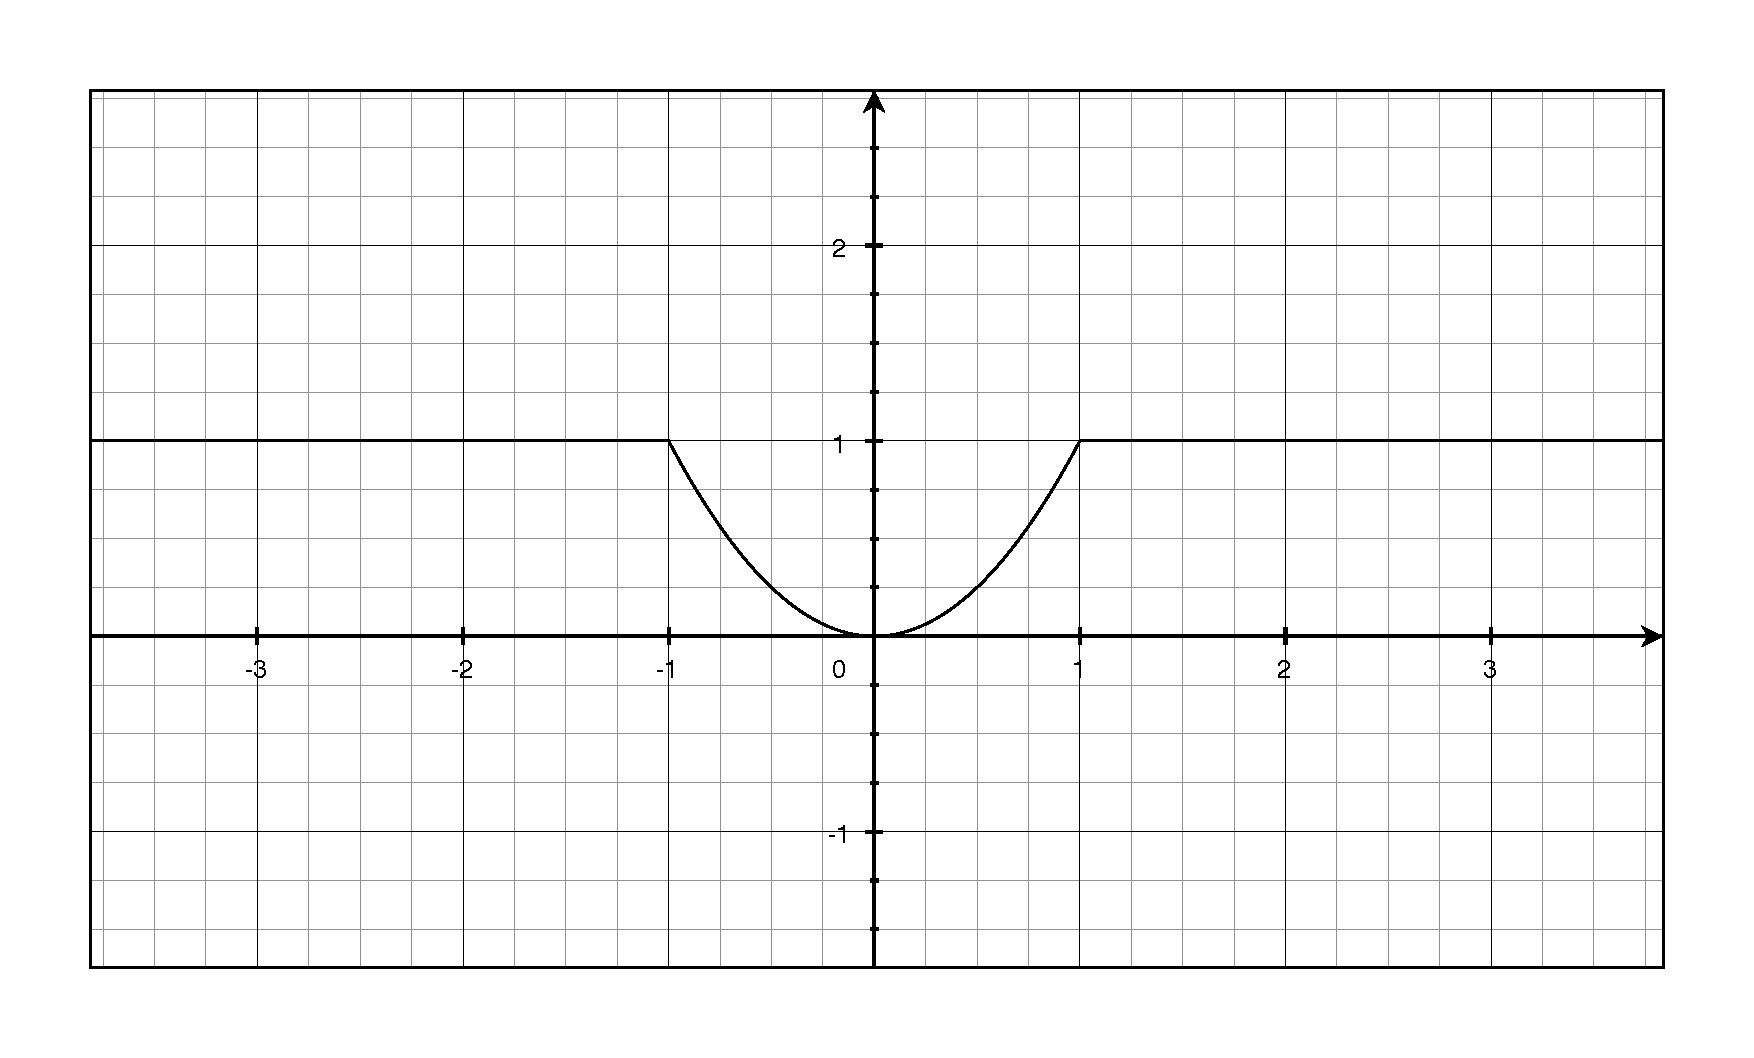
\includegraphics[scale = 0.8]{problem48.eps}
        \caption*{ Problem 48: $r(x) = \frac{4x^2}{x^2 - 2x - 3}$ }
      \end{figure}

    \item[49]
      \begin{tabular}{llll}
        \toprule
        x-intercept         & y-intercept & vertical          & horizontal \\
                            &             & asymptote         & asymptote \\
        \midrule
        $(-6, 0)$, $(1, 0)$ & $(0, 2)$    & $x = -3$, $x = 2$ & $y = 2$ \\
        \bottomrule
      \end{tabular}

      \begin{figure}[H]
        \centering
        \includegraphics[scale = 0.8]{problem49.eps}
        \caption*{ Problem 49: $r(x) = \frac{2x^2 + 10x - 12}{x^2 + x - 6}$ }
      \end{figure}

    \item[55]
      \begin{tabular}{llll}
        \toprule
        x-intercept & y-intercept & vertical         & horizontal \\
                    &             & asymptote        & asymptote \\
        \midrule
        $(1, 0)$    & none        & $x = 0$, $x = 3$ & $y = 0$ \\
        \bottomrule
      \end{tabular}

      \begin{figure}[H]
        \centering
        \includegraphics[scale = 0.8]{problem55.eps}
        \caption*{ Problem 55: $r(x) = \frac{x^2 - 2x + 1}{x^3 - 3x^2}$ }
      \end{figure}

    \item[56]
      \begin{tabular}{llll}
        \toprule
        x-intercept        & y-intercept & vertical          & horizontal \\
                           &             & asymptote         & asymptote \\
        \midrule
        $(0, 0)$, $(1, 0)$ & $(0, 0)$    & $x = -1$, $x = 2$ & $y = 1$ \\
        \bottomrule
      \end{tabular}

      \begin{figure}[H]
        \centering
        \includegraphics[scale = 0.8]{problem56.eps}
        \caption*{ Problem 56: $r(x) = \frac{x^3 - x^2}{x^3 - 3x - 2}$ }
      \end{figure}

    \item[57]
      \begin{tabular}{llll}
        \toprule
        x-intercept & y-intercept & vertical  & slant \\
                    &             & asymptote & asymptote \\
        \midrule
        $(0, 0)$    & $(0, 0)$    & $x = 2$   & $y = x + 2$ \\
        \bottomrule
      \end{tabular}

      \begin{figure}[H]
        \centering
        \includegraphics[scale = 0.8]{problem57.eps}
        \caption*{ Problem 57: $r(x) = \frac{x^2}{x - 2}$ }
      \end{figure}

    \item[58]
      \begin{tabular}{llll}
        \toprule
        x-intercept         & y-intercept & vertical  & slant \\
                            &             & asymptote & asymptote \\
        \midrule
        $(-2, 0)$, $(0, 0)$ & $(0, 0)$    & $x = 1$   & $y = x + 3$ \\
        \bottomrule
      \end{tabular}

      \begin{figure}[H]
        \centering
        \includegraphics[scale = 0.8]{problem58.eps}
        \caption*{ Problem 58: $r(x) = \frac{x^2 + 2x}{x - 1}$ }
      \end{figure}

    \item[59]
      \begin{tabular}{llll}
        \toprule
        x-intercept          & y-intercept & vertical  & slant \\
                             &             & asymptote & asymptote \\
        \midrule
        $(-2, 0)$, $(4, 0)$  & none        & $x = 0$   & $y = x - 2$ \\
        \bottomrule
      \end{tabular}

      \begin{figure}[H]
        \centering
        \includegraphics[scale = 0.8]{problem59.eps}
        \caption*{ Problem 59: $r(x) = \frac{x^2 - 2x - 8}{x}$ }
      \end{figure}

    \item[60]
      \begin{tabular}{llll}
        \toprule
        x-intercept        & y-intercept & vertical  & slant \\
                           &             & asymptote & asymptote \\
        \midrule
        $(0, 0)$, $(3, 0)$ & $(0, 0)$    & $x = 1$   & $y = - \frac{x}{2} + 1$ \\
        \bottomrule
      \end{tabular}

      \begin{figure}[H]
        \centering
        \includegraphics[scale = 0.8]{problem60.eps}
        \caption*{ Problem 60: $r(x) = \frac{3x - x^2}{x - 1}$ }
      \end{figure}

    \item[61]
      \begin{tabular}{llll}
        \toprule
        x-intercept          & y-intercept                       & vertical  & slant \\
                             &                                   & asymptote & asymptote \\
        \midrule
        $(-4, 0)$, $(-1, 0)$ & $\left( - \frac{4}{3}, 0 \right)$ & $x = 3$   & $y = x + 8$ \\
        \bottomrule
      \end{tabular}

      \begin{figure}[H]
        \centering
        \includegraphics[scale = 0.8]{problem61.eps}
        \caption*{ Problem 61: $r(x) = \frac{x^2 + 5x + 4}{x - 3}$ }
      \end{figure}

    \item[62]
      \begin{tabular}{llll}
        \toprule
        x-intercept                        & y-intercept & vertical                    & slant \\
                                           &             & asymptote                   & asymptote \\
        \midrule
        $ \left( - \sqrt[3]{4}, 0 \right)$ & $(0, -4)$   & $x = -1$, $x = \frac{1}{2}$ & $y = \frac{x}{2} - \frac{1}{4}$ \\
        \bottomrule
      \end{tabular}

      \begin{figure}[H]
        \centering
        \includegraphics[scale = 0.8]{problem62.eps}
        \caption*{ Problem 62: $r(x) = \frac{x^3 + 4}{2x^2 + x - 1}$ }
      \end{figure}

    \item[63]
      \begin{tabular}{llll}
        \toprule
        x-intercept         & y-intercept & vertical    & slant \\
                            &             & asymptote   & asymptote \\
        \midrule
        $(-1, 0)$, $(0, 0)$ & $(0, 0)$    & $x = -2$ and $x = 2$ & $y = x + 1$ \\
        \bottomrule
      \end{tabular}

      \begin{figure}[H]
        \centering
        \includegraphics[scale = 0.8]{problem63.eps}
        \caption*{ Problem 63: $r(x) = \frac{x^3 + x^2}{x^2 - 4}$ }
      \end{figure}

    \item[64]
      \begin{tabular}{llll}
        \toprule
        x-intercept & y-intercept & vertical    & slant \\
                    &             & asymptote   & asymptote \\
        \midrule
        $(0, 0)$    & $(0, 0)$    & $x = -1$ and $x = 1$ & $y = 2x$ \\
        \bottomrule
      \end{tabular}

      \begin{figure}[H]
        \centering
        \includegraphics[scale = 0.8]{problem64.eps}
        \caption*{ Problem 64: $r(x) = \frac{2x^3 + 2x}{x^2 - 1}$ }
      \end{figure}

    \pagebreak

    \item[81]
      \begin{enumerate}[a]
        \item 
          For a function to have a vertical asymptote at $x = 3$, it must have the factor $x - 3$ in its denominator.
          The simplest function that works is:
          \[
            r(x) = \frac{1}{x - 3}
          \]

          \begin{figure}[H]
            \centering
            \includegraphics{problem81a.eps}
            \caption*{Problem 81a: $r(x) = \frac{1}{x - 3}$}
          \end{figure}

        \pagebreak

        \item 
          For a function to have a vertical asymptote at $x = 3$ and a horizontal asymptote at $y = 2$:
          \begin{itemize*}
            \item it must have the factor $x - 3$ in its denominator
            \item the numerator and denominator must be the same degree
            \item the ratio of the leading coefficients in the numerator and denominator must be 2
          \end{itemize*}
          The simplest function that works is:
          \[
            r(x) = \frac{2x}{x - 3}
          \]

          \begin{figure}[H]
            \centering
            \includegraphics{problem81b.eps}
            \caption*{Problem 81b: $r(x) = \frac{2x}{x - 3}$}
          \end{figure}

        \pagebreak

        \item 
          For a function to have vertical asymptotes at $x = \pm 1$, a horizontal asymptote at $y = 0$, and an
          x-intercept at $x = 4$:
          \begin{itemize*}
            \item it must have the factors $x - 1$ and $x + 1$ in its denominator (vertical asymptotes)
            \item the denominator must be higher degree than the numerator (horizontal asymptote)
            \item the numerator must contain the factor $x - 4$ (x-intercept)
          \end{itemize*}
          The simplest function that works is:
          \[
            r(x) = \frac{x - 4}{x^2 - 1}
          \]
          \begin{figure}[H]
            \centering
            \includegraphics{problem81c.eps}
            \caption*{Problem 81c: $r(x) = \frac{x - 4}{x^2 - 1}$}
          \end{figure}
      \end{enumerate}
  \end{description}

\else
  \vspace{6 cm}
  \begin{quote}
    \begin{em}
      Well, if one really wishes to know how justice is administered in a country, one does not question the policemen,
      the lawyers, the judges, or the protected members of the middle class. One goes to the unprotected---those,
      precisely, who need the law's protection most!---and listens to their testimony. Ask any Mexican, any Puerto
      Rican, any black man, any poor person---ask the wretched how they fare in the halls of justice, and then you will
      know, not whether or not the country is just, but whether or not it has any love for justice, or any concept of
      it. It is certain, in any case, that ignorance, allied with power, is the most ferocious enemy justice can have.
    \end{em}
  \end{quote}

  \hspace{1 cm} --James Baldwin


\fi

\end{document}

